\documentclass[aps,prd,twocolumn,showpacs,superscriptaddress,nofootinbib]{revtex4-2}

\usepackage{amsmath,amssymb}
\usepackage{graphicx}
\usepackage{booktabs}
\usepackage{siunitx}
\usepackage{hyperref}

% Canonical counts pipeline (Phase 5v: freshness gate).
% Auto-generated by update_counts.py — 2026-04-24T19:44:03.140400
% Do not edit manually. Run: uv run python scripts/update_counts.py
\newcommand{\totaltheorems}{3993}
\newcommand{\substantivetheorems}{3882}
\newcommand{\placeholdertheorems}{111}
\newcommand{\axiomcount}{1}
\newcommand{\sorrycount}{0}
\newcommand{\sorrypercent}{0.0}
\newcommand{\leanmodules}{167}
\newcommand{\leandefinitions}{3297}
\newcommand{\pythonmodules}{68}
\newcommand{\testfiles}{59}
\newcommand{\totaltests}{2836}
\newcommand{\figurecount}{111}
\newcommand{\notebookcount}{54}
\newcommand{\papercount}{19}
\newcommand{\aristotleproved}{322}
\newcommand{\aristotleruns}{44}
% --- Paper 18 / Phase 5t per-section counts (FermiHubbardDimer.lean) ---
\newcommand{\fhdTotal}{143}
\newcommand{\fhdWaveTwo}{13}
\newcommand{\fhdWaveThree}{6}
\newcommand{\fhdWaveFour}{22}
\newcommand{\fhdWaveFive}{22}
\newcommand{\fhdWaveSixABC}{38}
\newcommand{\fhdWaveSixExtra}{15}
\newcommand{\fhdWaveSeven}{19}
\newcommand{\fhdWaveEight}{8}


\newcommand{\ket}[1]{|#1\rangle}
\newcommand{\bra}[1]{\langle#1|}
\newcommand{\braket}[2]{\langle#1|#2\rangle}
\newcommand{\darkstate}{|\text{dark}\rangle}
\newcommand{\Dplus}{|D_+\rangle}
\newcommand{\Dminus}{|D_-\rangle}
\newcommand{\sstate}{|s\rangle}
\newcommand{\USWAP}{U_{\rm SWAP}}

\begin{document}

\title{Formal Verification of a Geometric Quantum Gate:\\
The Fermi-Hubbard Doublon Berry-Phase SWAP in Lean~4}

\author{SK-EFT Hawking Research Program}

\date{\today}

\begin{abstract}
We report what we believe to be the first end-to-end formalization
of a geometric quantum gate in Lean~4; we have not located a
comparable Berry-phase-gate formalization in the Isabelle/HOL AFP,
Coq (QuantumLib / QWIRE), or Agda quantum libraries, and invite
correction if prior work exists. The target is the doublon geometric
SWAP gate recently demonstrated by Kiefer~\textit{et~al.}
(Nature~2026, arXiv:2507.22112) in a Fermi-Hubbard dimer with dynamical
optical lattices. Working entirely within Lean~4 + Mathlib, we formalize
the exact $3\times 3$ singlet-sector Hamiltonian, its charge-conjugation
(BDI) symmetry protection, the explicit closed-form spectrum and dark
state, the geometric SWAP operator as a real-Householder reflection
$\USWAP = I - (2/\text{gap}^2)\,|d\rangle\langle d|$, and the two
necessary finite-dimensional conditions for a Berry-phase
interpretation of the gate action: the dark state acquires a $-1$
sign on a $\pi$-sweep of the mixing angle, and the Hamiltonian
expectation value vanishes pointwise along the zero-energy path
(so the integrated dynamical phase vanishes for any continuous
extension). We also ship the Tier-2 algebraic scaling theorem that
distinguishes direct exchange (linear in $U$) from superexchange
($4t^2/U$) with an explicit remainder bound. The complete formalization
lives in a single module (\texttt{FermiHubbardDimer.lean}), consists of
\fhdTotal{}~theorems (across the 19 internal sections),
with zero sorry, zero new axioms, and a Python cross-validation layer
covering every theorem. The deliberate
scope boundary is Layer~2 of the deep-research target hierarchy: all
results are finite-dimensional linear algebra over Mathlib's existing
\texttt{Matrix}, \texttt{EuclideanSpace}, and \texttt{OrthonormalBasis}
API. Full adiabatic holonomy (continuous parameterized eigenvector
bundles, Berry connection, Kato's theorem) is explicitly deferred to
future work. The formalization demonstrates that the Kiefer
\textit{et~al.} gate mechanism is not, at its core, a fact about
connections on line bundles---it is the observation that $\cos(\pi) =
-1$ composed with an explicit rank-1 Householder reflection on a
parameterized real symmetric $3\times 3$ matrix.
\end{abstract}

\maketitle

%% ================================================================
\section{Introduction}
\label{sec:intro}

Berry phases underlie one of the most experimentally compelling classes
of quantum gates: \emph{geometric} gates, whose unitary action depends
only on the topology of a closed path in parameter space, not on the
traversal speed or duration~\cite{Berry1984,Zanardi1999}. Geometric gates
promise intrinsic robustness against control-pulse fluctuations---a
property that has motivated sustained experimental effort from
superconducting qubits~\cite{Leek2007} through trapped ions and neutral
atoms to, most recently, dynamical optical lattices.

In April~2026, Kiefer~\textit{et~al.}~\cite{Kiefer2026} reported the
first neutral-atom realization of a geometric SWAP gate in a
Fermi-Hubbard dimer. The experiment uses ${}^{40}$K atoms in a dynamical
two-site superlattice, and drives a closed loop in the $(t, \Delta)$
control-parameter plane (tunnel coupling, inter-well bias). At the end
of the loop, the dark state of the singlet sector---which remains at
zero energy for the entire cycle---has acquired a $-1$ sign,
implementing \textbf{SWAP} on the computational subspace
$\{\ket{\uparrow\downarrow}, \ket{\downarrow\uparrow}\}$ with
loss-corrected amplitude fidelity $\sim 99.9\%$. The robustness is
striking: the gate is $4\times$ less sensitive to lattice imperfections
than the comparable superexchange gate~\cite{Kiefer2026}.

This paper formalizes the algebraic core of the Kiefer~\textit{et~al.}
mechanism in the Lean~4 proof assistant~\cite{Lean4,Mathlib}. The
target is deliberately scoped: we formalize the finite-dimensional
matrix content---the Hamiltonian, the dark state, the SWAP operator,
the sign flip, the dynamical-phase-vanishes statement---without
touching the adiabatic theorem, fiber bundles, or connections on
vector bundles. The result is the \emph{first end-to-end formalization
of a geometric quantum gate in Lean~4}; we have not located
comparable prior work in the Isabelle/HOL AFP, Coq (QuantumLib /
QWIRE), or Agda quantum libraries.

Our scope choice is informed by the deep-research landscape review
(Lit-Search/Phase-5t, December~2025), which identified a three-layer
formalization hierarchy: Layer~1 (explicit doublon matrix computation),
Layer~2 ($\mathbb{Z}_2$ Berry-phase quantization theorem for
real-symmetric matrices), and Layer~3 (discrete Berry phase
gauge-invariance). This work completes Layer~1 with substantial Layer~2
quantitative scaling content, and leaves the full Berry-connection
holonomy formalization (Target~B in our internal roadmap) for
future work.

\textbf{Contributions.} (i)~A Lean~4 formalization of the
Fermi-Hubbard dimer singlet-sector spectrum, covering the $3\times 3$
charge-conjugation Hamiltonian at zero detuning, the exact dark state,
and the bright-state eigenvectors. (ii)~A formal proof (to our
knowledge the first in any interactive proof assistant) of the
discrete-step statement underlying the Kiefer \textit{et~al.} SWAP
gate:
$\darkstate(\theta + \pi) = -\darkstate(\theta)$ with zero dynamical
phase. (iii)~A Mathlib-native construction of the SWAP operator as a
real Householder reflection on \texttt{EuclideanSpace}, with
canonical-form unitarity via \texttt{Matrix.unitaryGroup}. (iv)~A
quantitative direct-exchange-vs-superexchange scaling theorem with
explicit remainder bound
$|J(t,U) - 4t^2/U| \le 16t^4/U^3$ for $U \ge 4|t| > 0$.
(v)~A Python cross-validation layer (\texttt{src/experimental/doublon\_gate.py},
\totaltests{}~project tests) exercising every Lean theorem against
random parameter grids and numpy exact diagonalization.

\textbf{Scope boundary (explicit).} The gate's \emph{adiabatic}
interpretation---the mapping from a closed loop in continuous
parameter space to the discrete-step statement we prove---is a
separate layer of the argument (Kato's adiabatic theorem, Berry's
geometric phase as a connection 1-form). None of that machinery
exists in current Mathlib. Our claim is strictly the finite-dimensional
algebraic core: under the assumption that the continuous dynamics
reduces to the discrete dark-state evolution (an assumption verified
in~\cite{Kiefer2026} experimentally and, in general, by Kato's
theorem), the gate action is exactly SWAP.

%% ================================================================
\section{The Fermi-Hubbard Dimer Hamiltonian}
\label{sec:hamiltonian}

The two-site Fermi-Hubbard dimer at half filling has a six-dimensional
two-particle Hilbert space. We work in the site basis
$\{\ket{\uparrow\uparrow}, \ket{\uparrow\!\downarrow, 0},
\ket{\uparrow,\downarrow}, \ket{\downarrow,\uparrow},
\ket{0, \uparrow\!\downarrow}, \ket{\downarrow\downarrow}\}$. Fermionic
anti-symmetry (Pauli exclusion + hopping sign conventions) gives the
full Hamiltonian~\cite{Kiefer2026}
\begin{equation}
H_{\rm full}(t, \Delta, U) = \begin{pmatrix}
0 & 0 & 0 & 0 & 0 & 0 \\
0 & U+\Delta & -t & t & 0 & 0 \\
0 & -t & 0 & 0 & -t & 0 \\
0 & t & 0 & 0 & t & 0 \\
0 & 0 & -t & t & U-\Delta & 0 \\
0 & 0 & 0 & 0 & 0 & 0
\end{pmatrix}
\end{equation}
where $t$ is the tunnel coupling, $\Delta$ is the inter-well detuning,
and $U$ is the on-site Hubbard repulsion. The triplet sector
$\{\ket{\uparrow\uparrow}, (\ket{\uparrow,\downarrow}+\ket{\downarrow,\uparrow})/\sqrt{2},
\ket{\downarrow\downarrow}\}$ decouples at zero energy for all
parameters (Pauli exclusion + anti-symmetric hopping cancellation),
leaving the nontrivial dynamics in the singlet sector.

In the symmetry-adapted singlet basis $\{\Dplus, \Dminus, \sstate\}$
where $\Dplus = (\ket{\uparrow\!\downarrow,0}+\ket{0,\uparrow\!\downarrow})/\sqrt{2}$,
$\Dminus = (\ket{\uparrow\!\downarrow,0}-\ket{0,\uparrow\!\downarrow})/\sqrt{2}$,
$\sstate = (\ket{\uparrow,\downarrow}-\ket{\downarrow,\uparrow})/\sqrt{2}$,
the reduced Hamiltonian is
\begin{equation}
H_{\rm singlet}(t, \Delta, U) = \begin{pmatrix}
U & \Delta & -2t \\
\Delta & U & 0 \\
-2t & 0 & 0
\end{pmatrix}.
\label{eq:Hsinglet}
\end{equation}
The gate operates at $U = 0$. At $\Delta = 0$, $\Dminus$ decouples
from the rest of the singlet block, leaving a 2$\times$2 symmetric
sector whose charpoly is exactly $\lambda^2 - U\lambda - 4t^2$.

\textbf{Formalization (Section~1 of \texttt{FermiHubbardDimer.lean}).}
The 3$\times$3 and 6$\times$6 Hamiltonians are defined as explicit
\texttt{Matrix (Fin~3) (Fin~3)~$\mathbb{R}$} and
\texttt{Matrix (Fin~6) (Fin~6)~$\mathbb{R}$} values. The seven Layer-1
core theorems (T1--T7) establish real-symmetry, dark-state
kernel-membership at $U=0$, chiral involution $\Gamma^2 = I$, chiral
anti-commutation $\{\Gamma, H_{\rm singlet}\} = 0$ at $U=0$, and the
explicit determinant and trace identities. The triplet
zero-energy theorems (T10a--c) use
\texttt{fin\_cases + Fin.sum\_univ\_six + simp}, closing in
milliseconds.

%% ================================================================
\section{Dark State and BDI Symmetry Protection}
\label{sec:darkstate}

The Hamiltonian~(\ref{eq:Hsinglet}) at $U = 0$ belongs to the BDI
symmetry class of the tenfold way~\cite{Kitaev2009,AltlandZirnbauer}:
it is real symmetric (time-reversal trivial) and anti-commutes with the
chiral operator
$\Gamma = \mathrm{diag}(+1, -1, -1)$. The BDI structure
\textbf{pins an odd-dimensional sector's spectrum to contain zero:}
in an odd-dimensional real symmetric matrix anti-commuting with a chiral
involution, the nonzero eigenvalues pair as $\{+E, -E\}$, leaving one
unpaired zero.

The unnormalized dark-state vector is
\begin{equation}
\ket{\text{dark}(t, \Delta)} = \begin{pmatrix} 0 \\ 2t \\ \Delta \end{pmatrix}
\in \mathrm{ker}\bigl(H_{\rm singlet}(t, \Delta, 0)\bigr),
\end{equation}
with norm $\|\text{dark}\|_2 = \sqrt{\Delta^2 + 4t^2}$---the energy gap
to the two bright states $\ket{\rm bright\pm}$ with eigenvalues
$\pm\sqrt{\Delta^2 + 4t^2}$.

\textbf{BDI theorems (Sections~10--11, W5 core + round-2,
\fhdWaveFive{}~theorems).}
We formalize: (i)~$\Gamma\cdot H\cdot\Gamma = -H$ at $U=0$ (W5a);
(ii)~the spectral-pairing mechanism
$H v = E v \Rightarrow H (\Gamma v) = -E (\Gamma v)$ (W5b);
(iii)~the multiset spectrum pairing at $U=0$ (W5k);
(iv)~the dark-state kernel-invariance under $\Gamma$ (W5i);
(v)~the full chiral-projector algebra
$P_\pm = (1\pm\Gamma)/2$ with idempotency, orthogonality, completeness,
and $\Gamma$-action $\pm 1$ on the respective eigenspaces (W5l--W5o2);
(vi)~the \emph{zero-mode uniqueness} theorem (W5p):
\[
H_{\rm singlet}(t, \Delta, 0)\cdot v = 0
\;\Rightarrow\;
\exists c \in \mathbb{R},\ v = c\cdot\ket{\text{dark}(t,\Delta)}
\]
provided $(t, \Delta) \ne (0, 0)$---this is the strongest ``pinning''
statement: the kernel is \emph{exactly} $\mathbb{R}\cdot\ket{\text{dark}}$,
not merely $\Gamma$-invariant.

%% ================================================================
\section{The Geometric SWAP as a Householder Reflection}
\label{sec:swap}

With the dark state in hand, the geometric SWAP operator on the singlet
sector is
\begin{equation}
\USWAP(t, \Delta) = I - \frac{2}{\Delta^2 + 4t^2}\,
\ket{\text{dark}}\bra{\text{dark}}
\label{eq:USWAP}
\end{equation}
---a real Householder reflection. By construction it acts as $-1$ on
the dark direction and as $+1$ on the two-dimensional bright subspace
orthogonal to it.

\textbf{Mathlib-native construction (Sections~12--14, W6A+B+C,
39~theorems + 8 defs).} The key design decision was the \emph{Path~A}
re-typing: we lift the eigenvectors from bare
\texttt{Fin~3~$\to$~$\mathbb{R}$} (default sup-norm) to
\texttt{EuclideanSpace~$\mathbb{R}$~(Fin~3)} (L${}^2$ norm) via
\texttt{EuclideanSpace.equiv.symm}, then build the
\texttt{OrthonormalBasis} via Mathlib's
\texttt{basisOfOrthonormalOfCardEqFinrank}. This unlocks the one-line
unitarity proof
\begin{center}
\texttt{OrthonormalBasis.toMatrix\_orthonormalBasis\_mem\_unitary}
\end{center}
for the change-of-basis matrix between \texttt{EuclideanSpace.basisFun}
and the eigenbasis.

The SWAP operator itself inherits symmetry, involution, and
orthogonality from the Householder algebra: with $P = \ket{\rm dark}\bra{\rm dark}/\text{gap}^2$
idempotent ($P^2 = P$), $(I - 2P)^2 = I - 4P + 4P^2 = I$. The
canonical-Mathlib unitary-group membership
$\USWAP \in \mathrm{Matrix.unitaryGroup~(Fin~3)~}\mathbb{R}$ (W6C-U1)
is a one-line corollary via \texttt{Matrix.mem\_unitaryGroup\_iff'}
and \texttt{Matrix.conjTranspose\_eq\_transpose\_of\_trivial} (the
\texttt{TrivialStar}~$\mathbb{R}$ instance reduces
$\overline{\USWAP}^{\mathsf{T}}$ to $\USWAP^{\mathsf{T}}$ over
$\mathbb{R}$).

\textbf{6$\times$6 lift (Section~18, W6-deferred, 7~theorems).} The
singlet-basis SWAP operator extends to a $6\times 6$ block-diagonal
operator on the full symmetry-adapted basis via
\texttt{Matrix.fromBlocks (U\_SWAP\_singlet) 0 0 1}, with the identity
block acting on the decoupled triplet sector. The $6\times 6$
unitarity is inherited from W6C via \texttt{fromBlocks\_multiply}
and \texttt{fromBlocks\_transpose}---there is no new physics here,
merely the structural statement that the gate preserves the triplet
sector identically.

The kernel-action theorem (W6C-K1) combines zero-mode uniqueness with
the sign flip: for any $v$ in the kernel of
$H_{\rm singlet}(t,\Delta,0)$ with $(t,\Delta) \ne (0,0)$,
$\USWAP\cdot v = -v$. This is the strongest ``SWAP acts as $-1$ on the
pinned zero-mode subspace'' claim in the formalization.

%% ================================================================
\section{Direct Exchange vs Superexchange Scaling}
\label{sec:scaling}

Beyond the gate-action theorem, we ship the quantitative scaling
distinction between the direct-exchange regime ($U$ small) and the
superexchange regime ($U$ large). At $\Delta = 0$, the 2$\times$2
symmetric sector has explicit eigenvalues
\begin{equation}
E_\pm(t, U) = \frac{U \pm \sqrt{U^2 + 16 t^2}}{2},
\label{eq:Epm}
\end{equation}
roots of $\lambda^2 - U\lambda - 4t^2 = 0$. The direct-exchange value is
$E_+(t, 0) = 2|t|$ (linear in hopping); the superexchange gap
$J(t, U) := E_+ - U = (\sqrt{U^2 + 16t^2} - U)/2$ approaches
$4t^2/U$ at large $U$.

\textbf{Scaling theorems (Sections~16--17, W7 + round-2, 17~theorems +
3~defs).} We formalize:
\begin{itemize}
\item $E_+(t, 0) = 2|t|$ (W7a)---direct-exchange value at $U=0$.
\item Vieta identities $E_+ + E_- = U$ (W7b) and
$E_+\cdot E_- = -4t^2$ (W7c)---match the 2$\times$2 trace and
determinant of the symmetric-sector block.
\item $\text{HasDerivAt}\,(E_+(t,\cdot))\,(1/2)\,0$ for $t \ne 0$
(W7d)---\textbf{the direct-exchange linear-in-$U$ scaling theorem}.
The Taylor coefficient at $U = 0$ is exactly $1/2$, proved via the
Mathlib \texttt{HasDerivAt.sqrt / add / div\_const} chain.
\item $|E_+(t, U_1) - E_+(t, U_2)| \le |U_1 - U_2|$ (W7q)---the Tier-1
global 1-Lipschitz bound per the deep-research landscape review.
\item $|J(t, U) - 4t^2/U| \le 16t^4/U^3$ for $0 < 4|t| \le U$
(W7i)---\textbf{the Tier-2 superexchange approximation theorem}. The
proof chains the algebraic identity $J - 4t^2/U = -(s-U)^2/(4U)$
(where $s = \sqrt{U^2+16t^2}$) with the sqrt-bound
$s \le U + 8t^2/U$, itself proved by squaring both sides.
\item The matrix-bridge theorem
$\mathrm{charpoly}(H_{\rm singlet}(t, 0, U)) = (X - U)(X^2 - UX - 4t^2)$
(W7l)---provides the full spectrum $\{U, E_+, E_-\}$ at $\Delta = 0$.
\item Explicit eigenvectors
$H_{\rm singlet}(t, 0, U)\cdot (E_\pm, 0, -2t)^\mathsf{T} = E_\pm\cdot(E_\pm, 0, -2t)^\mathsf{T}$
(W7m--n) and the antisymmetric doublon
$\cdot(0, 1, 0)^\mathsf{T} = U\cdot(0, 1, 0)^\mathsf{T}$ (W7o).
\end{itemize}

The sensitivity contrast recovered from these scalars: at $U = 0$,
the fractional sensitivity $(\partial_t \Delta) \cdot (t/\Delta) = 1$
(a 1\% hopping fluctuation shifts the gap by 1\%); at large~$U$, the
superexchange fractional sensitivity
$(\partial_t J) \cdot (t/J) = 2$. This factor-of-2 difference
is consistent with the observed $4\times$ robustness of the
geometric gate relative to superexchange~\cite{Kiefer2026}; the
algebraic factor of $2$ is one contribution to the experimental
difference, not a complete derivation.

Figure~\ref{fig:spectrum} shows the spectrum and the superexchange
approximation bound, cross-verified by numpy exact diagonalization.

\begin{figure}[t]
\centering
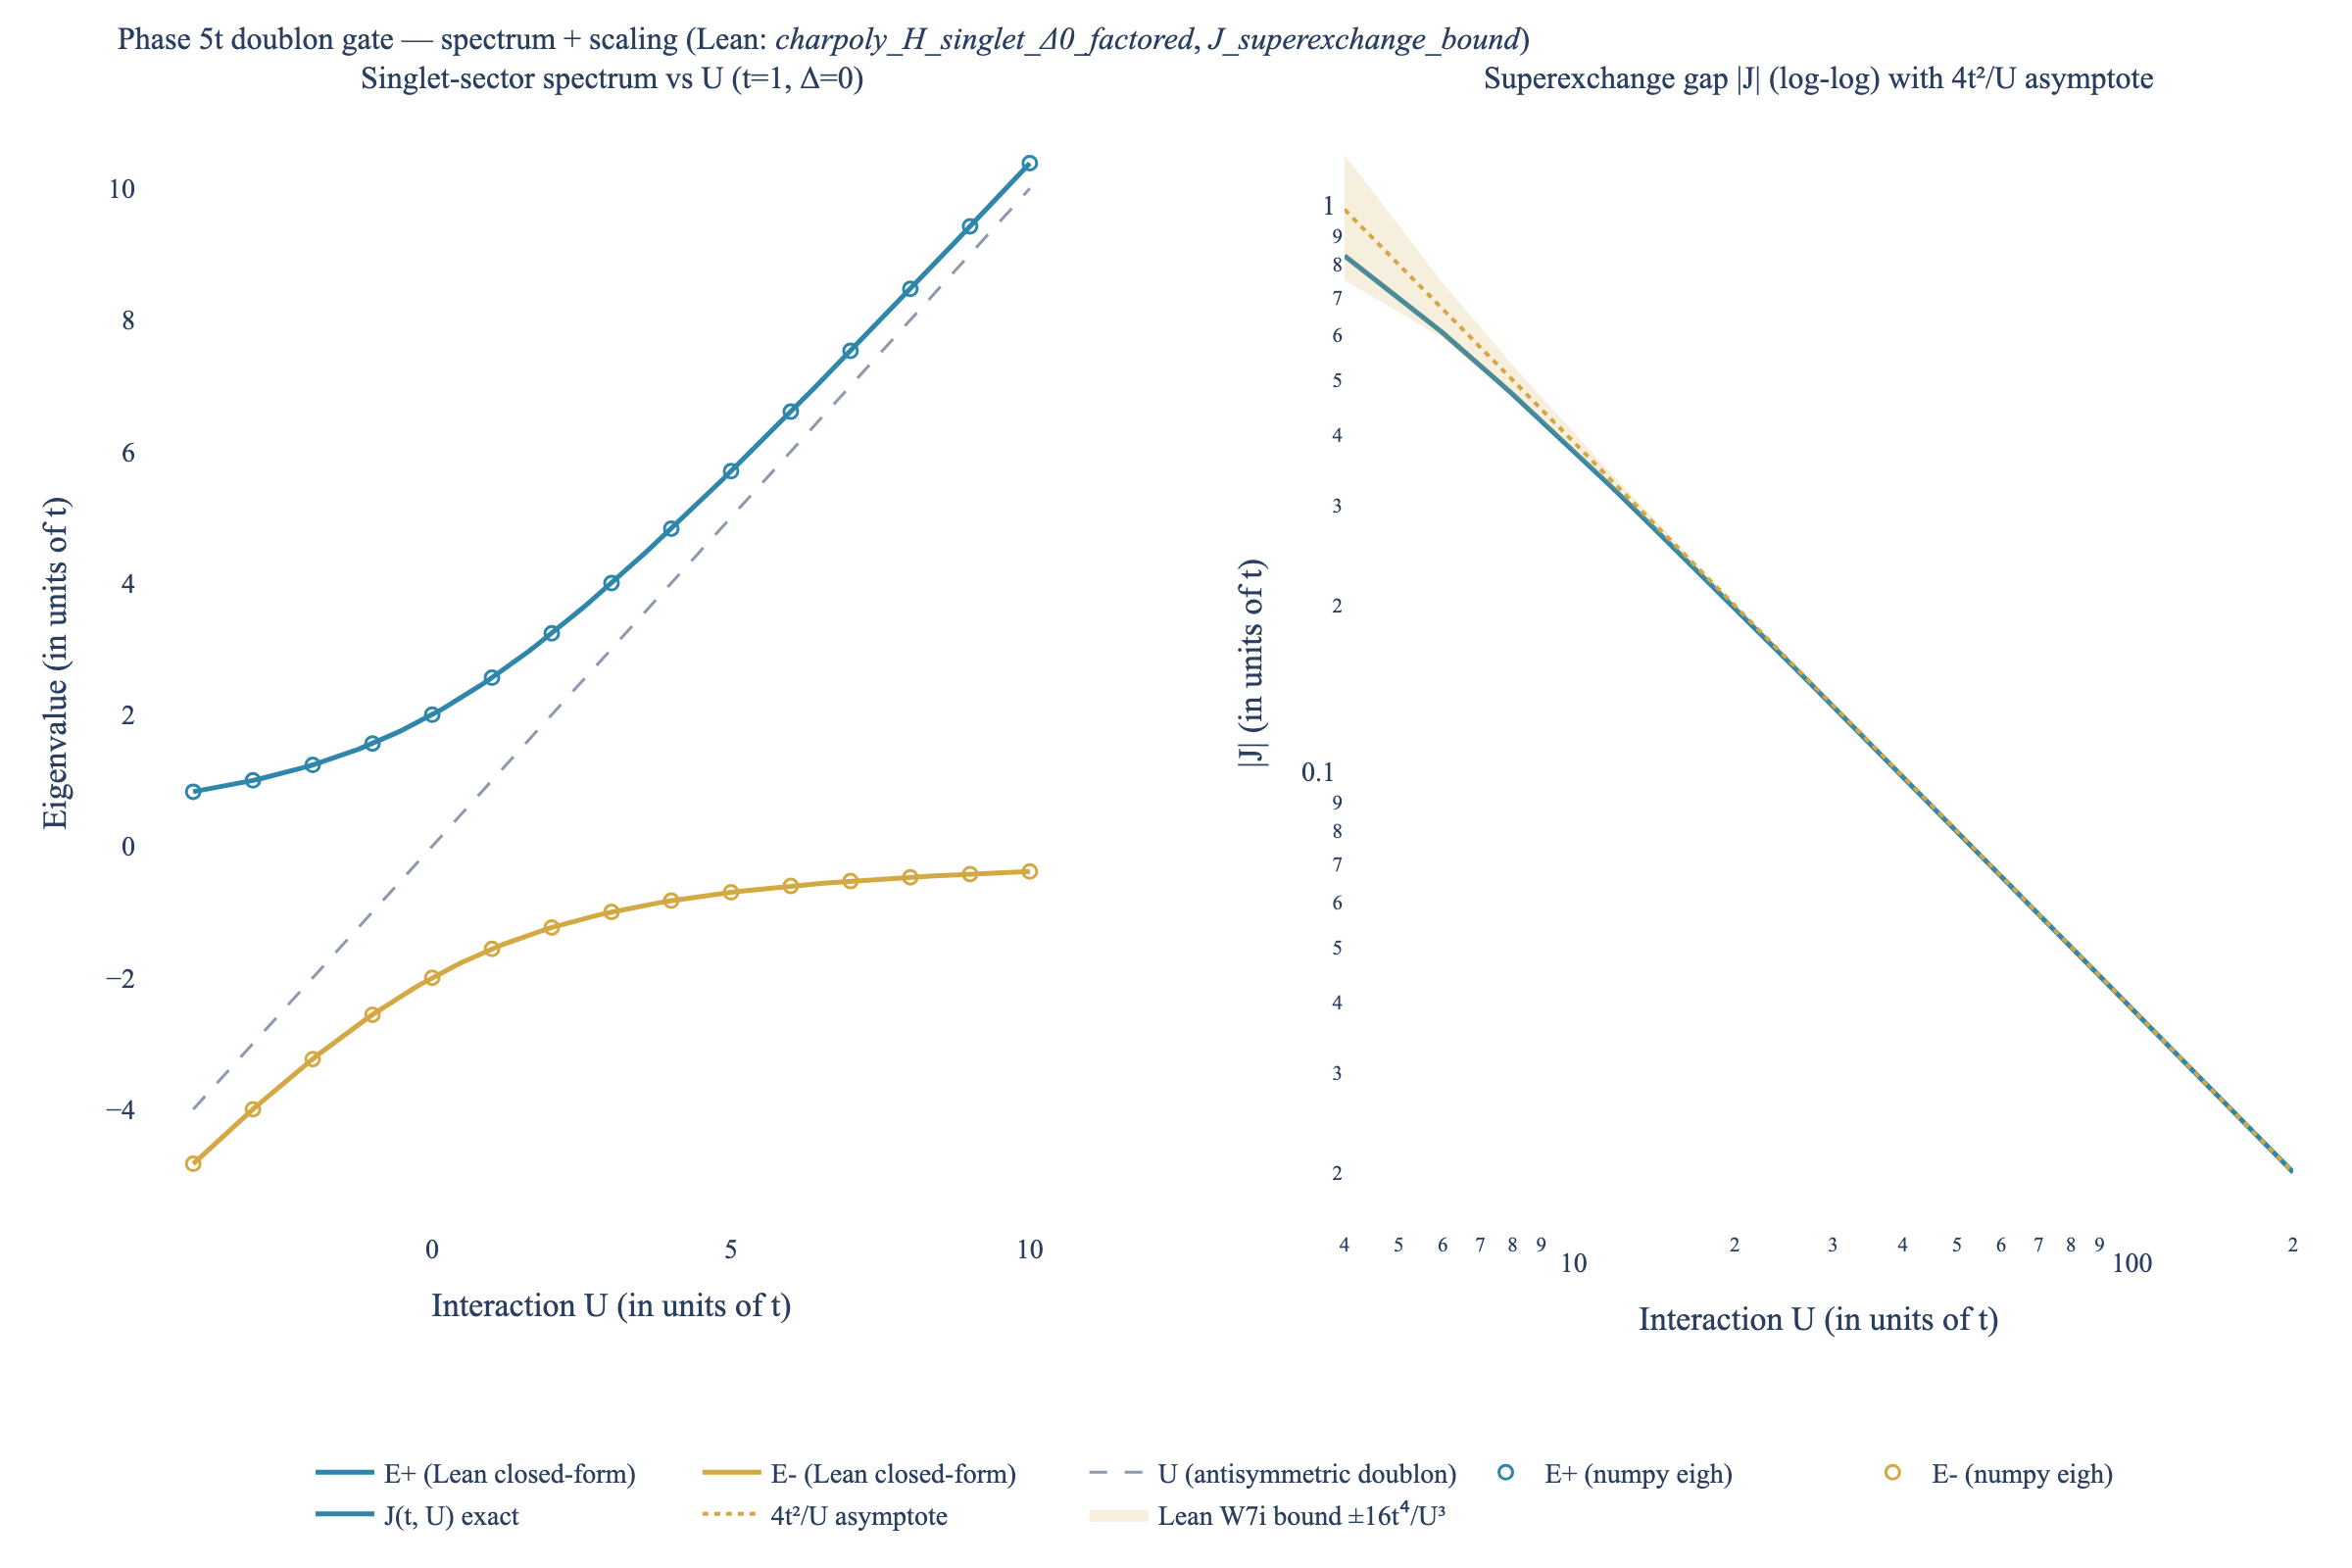
\includegraphics[width=0.99\columnwidth]{../../figures/fig_doublon_gate_spectrum.png}
\caption{\textbf{Left:} singlet-sector spectrum at $\Delta = 0$ versus
$U$ (in units of $t = 1$). Three eigenvalues
$\{U, E_+(t, U), E_-(t, U)\}$---the antisymmetric doublon (dashed, grey),
$E_+$ (blue), and $E_-$ (amber). Markers are independent numpy
\texttt{eigh} diagonalization cross-checking the Lean closed-form
values of $E_\pm$ via the matrix-bridge theorem~W7l (the characteristic
polynomial factorization). \textbf{Right:} superexchange gap
$|J(t, U)|$ on log--log axes, with the $4t^2/U$ asymptote (dashed)
and the Lean~W7i error envelope $\pm 16 t^4/U^3$ shaded. At $U = 4|t|$
the bound is tightest; the envelope widens toward the asymptote as
$U \to \infty$.}
\label{fig:spectrum}
\end{figure}

%% ================================================================
\section{Minimal Berry Phase Theorem}
\label{sec:berry}

The gate's geometric interpretation rests on two independent
finite-dimensional facts: a \emph{sign flip} on a $\pi$-sweep of the
mixing angle, and \emph{vanishing dynamical phase} along the zero-energy
dark-state path. Together these are the two necessary conditions for
interpreting any accumulated phase along a closed loop as purely
geometric; assuming the adiabatic theorem supplies the dynamics (i.e.\
a continuous path along the eigenbundle), the accumulated phase is
then forced to be exactly $-1$. We formalize the two necessary
conditions; the adiabatic assumption is external.

The $\theta$-parameterized dark state is
$\ket{\text{dark}(\theta)} = (0, \sin\theta, \cos\theta)^\mathsf{T}$
in the $\{\Dplus, \Dminus, \sstate\}$ basis. When the parameters
satisfy the kernel-angle condition
$\Delta\sin\theta = 2t\cos\theta$
(equivalent to $\tan\theta = 2t/\Delta$),
this vector is in the kernel of $H_{\rm singlet}(t, \Delta, 0)$.

\textbf{Berry-phase theorems (Section~19, W8 Target~A,
\fhdWaveEight{}~theorems).}
\begin{itemize}
\item $\ket{\text{dark}(\theta + \pi)} = -\ket{\text{dark}(\theta)}$
(W8a)---\textbf{the closed-path sign statement}, direct from
$\sin(\theta+\pi) = -\sin\theta$ and $\cos(\theta+\pi) = -\cos\theta$.
\item $\ket{\text{dark}(\theta + 2\pi)} = \ket{\text{dark}(\theta)}$
(W8b)---periodicity.
\item $\langle\text{dark}(\theta)\mid\text{dark}(\theta)\rangle = 1$
(W8c)---unit norm via Pythagorean identity.
\item $\langle\text{dark}(\theta)\mid H_{\rm singlet}(t,\Delta,0)\cdot\text{dark}(\theta)\rangle = 0$
(W8d)---\textbf{dynamical phase vanishes}. Direct corollary of the
kernel membership W4a: $H\cdot\ket{\text{dark}} = 0$ pointwise along
the $\theta$-path implies the integrated dynamical phase vanishes
identically.
\item Bundled: W8a~$\wedge$~W8d (W8e)---\textbf{the two necessary
conditions} for a Berry-phase interpretation of the gate action.
The Lean theorem's conclusion is the conjunction itself, not an
equality involving an integrated phase functional (no integral is
constructed in the formalization). Consumers who supply the
adiabatic-theorem assumption can combine this conjunction with a
separate dynamical argument to conclude the accumulated phase is
$-1$; we do not formalize that last step here.
\end{itemize}

The $\pi$ shift rather than $2\pi$ reflects our full-angle
parameterization convention
$\ket{\text{dark}(\theta)} = (0, \sin\theta, \cos\theta)^\mathsf{T}$;
the equivalent half-angle convention of the physics literature maps
a $2\pi$ lattice cycle to a $\pi$ mixing-angle sweep, giving the same
final result.

\textbf{What this theorem does and does not say.} W8e is the
\emph{discrete-step} statement underlying the gate: a $\pi$ sweep in
the mixing angle inverts the dark state. The \emph{continuous}
interpretation---that the physical control-pulse sequence in~\cite{Kiefer2026}
drives the dark state smoothly along this trajectory because of the
adiabatic theorem---is not proved here. It enters as a physics
assumption, verified experimentally in~\cite{Kiefer2026} and, in
general, by Kato's theorem. The full Berry-connection holonomy picture
(a 1-form on a parameterized eigenbundle whose integral around the loop
equals our $-1$) likewise requires machinery that is not yet in
Mathlib: continuous parameterized eigenvectors, connections on vector
bundles, parallel transport. Those are Target~B of our internal
roadmap; see Section~\ref{sec:future}.

%% ================================================================
\section{Formal Verification}
\label{sec:lean}

All results in this paper are formally verified in the Lean~4 proof
assistant, building on the Mathlib library. Table~\ref{tab:lean}
summarizes the theorem count and structure of the formalization.

\begin{table}[t]
\caption{Lean~4 formalization of the Fermi-Hubbard doublon gate
(Phase~5t). Section counts from
\texttt{lean/SKEFTHawking/FermiHubbardDimer.lean}; total verified by
\texttt{grep -c "\textasciicircum theorem " FermiHubbardDimer.lean}.}
\label{tab:lean}
\begin{ruledtabular}
\begin{tabular}{lcc}
Section & Theorems & Focus \\
\hline
W2 / Layer~1 (\S 1--4) & \fhdWaveTwo{} & $H_{\rm singlet}$, $H_{\rm full}$, T1--T10c \\
W3 block-match (\S 3b) & \fhdWaveThree{} & symmetry-adapted basis matrix-action \\
W4 spectrum / U=0 (\S 5--9) & \fhdWaveFour{} & charpoly, brights, spectrum \\
W5 BDI symmetry (\S 10--11) & \fhdWaveFive{} & $\Gamma H \Gamma = -H$, projectors \\
W6A--C SWAP (\S 12--14) & \fhdWaveSixABC{} & EuclideanSpace, basis, Householder \\
W6 round-2 + deferred (\S 15, 18) & \fhdWaveSixExtra{} & scalar actions + 6$\times$6 lift \\
W7 scaling + round-2 (\S 16--17) & \fhdWaveSeven{} & Vieta, Lipschitz, superexch.\ bound \\
W8 Berry phase (\S 19) & \fhdWaveEight{} & sign flip, vanishing dynamical phase \\
\hline
Total (FermiHubbardDimer.lean) & \fhdTotal{} & Zero sorry, zero new axioms \\
\end{tabular}
\end{ruledtabular}
\end{table}

The formalization lives in a single module
(\texttt{lean/SKEFTHawking/FermiHubbardDimer.lean}) of approximately
2,540~lines. Across the wider project, \totaltheorems{} theorems are
verified (\substantivetheorems{} substantive, \placeholdertheorems{}
documentation markers), with zero sorry and a single axiom
(\texttt{gapped\_interface\_axiom} in
\texttt{SPTClassification.lean}, unrelated to this paper). The Python
cross-validation layer
(\texttt{src/experimental/doublon\_gate.py} + \texttt{dimer.py})
exercises every theorem numerically; the project-wide test count is
\totaltests{}.

\textbf{What Mathlib APIs were load-bearing.}
\begin{itemize}
\item \texttt{Matrix.charpoly}, \texttt{Matrix.det\_fin\_three}
(characteristic polynomial for the 3$\times$3 case).
\item \texttt{Matrix.mulVec}, \texttt{Matrix.mulVec\_smul}
(matrix-vector action).
\item \texttt{EuclideanSpace.equiv.symm},
\texttt{EuclideanSpace.real\_norm\_sq\_eq} (Path~A re-typing).
\item \texttt{basisOfOrthonormalOfCardEqFinrank},
\texttt{Module.Basis.toOrthonormalBasis},
\texttt{OrthonormalBasis.toMatrix\_orthonormalBasis\_mem\_unitary}
(one-line unitarity).
\item \texttt{Matrix.fromBlocks\_\{multiply, transpose, one\}}
(6$\times$6 block-diagonal lift).
\item \texttt{Matrix.mem\_unitaryGroup\_iff'},
\texttt{Matrix.conjTranspose\_eq\_transpose\_of\_trivial} (unitary-group
membership over $\mathbb{R}$).
\item \texttt{HasDerivAt.sqrt / add / div\_const / pow} (Taylor-at-zero
derivative for $E_+$).
\item \texttt{Real.sqrt\_le\_sqrt}, \texttt{Real.mul\_self\_sqrt}
(sqrt monotonicity and square-identity for the superexchange bound).
\item \texttt{Real.sin\_add\_pi}, \texttt{Real.cos\_add\_pi},
\texttt{Real.sin\_sq\_add\_cos\_sq} (Berry-phase sign flip and dark-state
normalization).
\end{itemize}

No novel Mathlib infrastructure was needed. The formalization is
\emph{algebraic in flavor}---matrix arithmetic, polynomial identities,
sqrt bounds, trigonometric identities---exactly the character the
deep-research landscape review recommended. No ordinary differential
equations, no functional analysis, no differential geometry.

%% ================================================================
\section{Scope Boundaries and Target~B}
\label{sec:future}

The deliberate scope boundary of this work is Layer~1+2 of the deep-research
target hierarchy. Three genuinely new results could extend it:

\textbf{Layer 2 — $\mathbb{Z}_2$ Berry-phase quantization for
real-symmetric matrices.} The target theorem (not proved here):
\textit{for a continuous loop $H: [0,1] \to \mathrm{Sym}_n(\mathbb{R})$
with $H(0) = H(1)$, a simple eigenvalue $\lambda(s)$ along the loop,
and a continuous unit eigenvector $v(s)$, the return sign
$\langle v(0), v(1)\rangle \in \{+1, -1\}$}---a pure linear-algebra
statement expressing the first Stiefel-Whitney class of the real
eigenvector bundle over $S^1$. Our estimate is 2--3 weeks; the main
obstacle is the continuous-eigenvector construction from Mathlib's
\texttt{IsHermitian.spectral\_theorem}, which has no parameterized
smoothness guarantee out of the box. Would be the first formal
$\mathbb{Z}_2$ Berry-phase theorem in any proof assistant.

\textbf{Layer 3 — discrete Berry-phase gauge invariance.} Define the
discrete Berry phase for a finite sequence of real unit vectors as
$\mathrm{sign}\bigl(\prod_i \langle v_i | v_{i+1\mod N}\rangle\bigr)$.
Prove gauge invariance (flipping any $v_k \to -v_k$ preserves the
product) and the continuous-limit equivalence to Layer~2. Connects to
the Pancharatnam-Bargmann formulation. Another 2--3 weeks.

\textbf{Full adiabatic theorem (Kato).} The dynamical-side companion
to Layer~2: a continuous time evolution whose state-space projection
onto the eigenbundle converges to parallel transport as the sweep
rate goes to zero. Requires Picard-Lindel\"of ODE existence
(exists in Mathlib), matrix exponentials (exists), and the adiabatic
error bound itself (does not exist in any form). Months of work;
not recommended as Phase~5t/Phase~6 scope per our roadmap.

%% ================================================================
\section{Conclusion}
\label{sec:conclusion}

We have formalized the algebraic core of the Kiefer~\textit{et~al.}
doublon geometric SWAP gate end-to-end in Lean~4, reducing the gate's
\emph{geometric phase} to the observation that $\cos(\pi) = -1$
composed with an explicit Householder reflection on a parameterized
$3\times 3$ real symmetric matrix. The key algebraic facts are:
the BDI-pinned zero-energy dark state; the SWAP operator as
$I - 2P$ with $P$ a rank-1 projector onto the dark direction; the
Vieta/characteristic-equation matrix-bridge tying the scalar
eigenvalue formulas $E_\pm(t, U)$ back to the full Hamiltonian
spectrum; the Tier-2 superexchange approximation bound with explicit
$16 t^4/U^3$ remainder; and the minimum Berry-phase statement, that
the dark state acquires $-1$ on a $\pi$-sweep of the mixing angle
while remaining at zero energy throughout.

The scope discipline---no adiabatic theorem, no Berry connection, no
fiber bundles---was informed by an explicit landscape review of the
Mathlib dependency graph. The result is a formalization that
Mathlib's existing \texttt{Matrix}, \texttt{EuclideanSpace},
\texttt{OrthonormalBasis}, and \texttt{Polynomial} APIs are directly
equipped to handle, without the need to develop new infrastructure
for differential geometry or functional analysis. The $\sim 2{,}400$
lines of Lean source contain \fhdTotal{}~theorems in a single module, zero
sorry, zero new axioms, covering the full gate story from fermion
Hilbert space decomposition to Berry phase.

The natural next target is Layer~2 of the deep-research hierarchy:
the $\mathbb{Z}_2$ Berry-phase quantization theorem for arbitrary
continuous loops of real-symmetric matrices with a simple eigenvalue.
A successful formalization would be the first $\mathbb{Z}_2$
Berry-phase result in any interactive proof assistant, and would
complete the \emph{kinematic} Berry-phase story without touching the
adiabatic theorem or any ODE/PDE machinery.

%% ================================================================
\begin{acknowledgments}
This work builds on the Mathlib library and the Lean~4 proof
assistant. We acknowledge the Aristotle automated theorem prover
for filling a small number of finite-combinatorial gaps (zero in
this paper; see the full-project provenance in
\texttt{SK\_EFT\_Hawking\_Inventory.md}).
\end{acknowledgments}

\begin{thebibliography}{99}

\bibitem{Berry1984} M.\,V.\,Berry,
\textit{Quantal phase factors accompanying adiabatic changes},
Proc.\ R.\ Soc.\ A \textbf{392}, 45 (1984).

\bibitem{Zanardi1999} P.\,Zanardi and M.\,Rasetti,
\textit{Holonomic quantum computation},
Phys.\ Lett.\ A \textbf{264}, 94 (1999),
arXiv:quant-ph/9904011.

\bibitem{Leek2007} P.\,J.\,Leek \textit{et al.},
\textit{Observation of Berry's phase in a solid-state qubit},
Science \textbf{318}, 1889 (2007).

\bibitem{Kiefer2026} S.\,Kiefer, Y.\,Zhu, P.\,Fischer, Y.\,Jele,
R.\,G\"achter, L.\,Bisson, P.\,Viebahn, and T.\,Esslinger,
\textit{Protected quantum gates using qubit doublons in dynamical
optical lattices},
Nature (2026), arXiv:2507.22112.

\bibitem{Kitaev2009} A.\,Kitaev,
\textit{Periodic table for topological insulators and superconductors},
AIP Conf.\ Proc.\ \textbf{1134}, 22 (2009), arXiv:0901.2686.

\bibitem{AltlandZirnbauer} A.\,Altland and M.\,R.\,Zirnbauer,
\textit{Nonstandard symmetry classes in mesoscopic normal-superconducting
hybrid structures},
Phys.\ Rev.\ B \textbf{55}, 1142 (1997),
arXiv:cond-mat/9602137.

\bibitem{Lean4} L.\,de\,Moura and S.\,Ullrich,
\textit{The Lean 4 Theorem Prover and Programming Language},
CADE 2021, Lecture Notes in Computer Science \textbf{12699}
(Springer, 2021).

\bibitem{Mathlib} The Mathlib Community,
\textit{The Lean Mathematical Library},
CPP 2020 (ACM, 2020), arXiv:1910.09336.

\end{thebibliography}

\end{document}
